\documentclass[10pt,a4paper]{article}
\usepackage[margin=21mm,headheight=15pt]{geometry}
\usepackage[T1]{fontenc}
\usepackage{lmodern,amsmath,amssymb,tikz,graphicx,hyperref,fancyhdr,enumitem}
\usetikzlibrary{arrows.meta,positioning,calc,decorations.pathmorphing}
\definecolor{ink}{RGB}{20,53,78}
\hypersetup{colorlinks=true,urlcolor=ink,linkcolor=ink}
\setlength{\parindent}{0pt}\setlength{\parskip}{5pt}
\emergencystretch=3em
\pagestyle{fancy}\fancyhf{}\fancyfoot[C]{\thepage}
\renewcommand{\headrulewidth}{.3pt}
\newcommand{\task}[2]{\par\medskip{\color{ink}\Large\bfseries #1. #2}\par\smallskip}
\newcommand{\answer}{\par\smallskip\textbf{Worked reasoning.} }
\setlist[enumerate]{label=\textbf{(\alph*)},leftmargin=7mm,itemsep=7pt}
\begin{document}
\fancyhead[L]{\small Control of Dynamical Systems}
\fancyhead[R]{\small Laboratory 02}
{\color{ink}\LARGE\bfseries Laboratory 02}\par
{\large Ventilation as a bilinear dynamical system}\par
\textbf{Exercise sheet -- five integrated problems}\par
{\small\textbf{Evidence boundary.} Original hypothetical scenarios. Derive, calculate and justify decisions; every numerical record is synthetic. Figures are conceptual and not to scale.}
\smallskip\textbf{Shared nominal data.} Nominal room: $V=120$ m$^3$, source $S=360$ ppm m$^3$/min and ventilation $q_0=3$ m$^3$/min, with clean inlet air and perfect mixing. Excess concentration $c$ is in ppm. Problem 5 introduces a separate liquid analogue with explicitly different units.
\par\smallskip{\small\textbf{Study route.} On a first modeling pass, solve Problems 1--3 and 5(b). Return to Problem 4 and 5(a,c) after Laboratory 05 introduces PI feedback; revisit actuator limits after Laboratory 09.}
\task{1}{From a ventilated room to a local input--output model}
A room has a uniform excess tracer concentration. Fresh air removes tracer, and a separate source generates it. Distinguish airflow from tracer flow in the physical illustration.
\begin{center}\resizebox{\ifdim\width>.98\linewidth.98\linewidth\else\width\fi}{!}{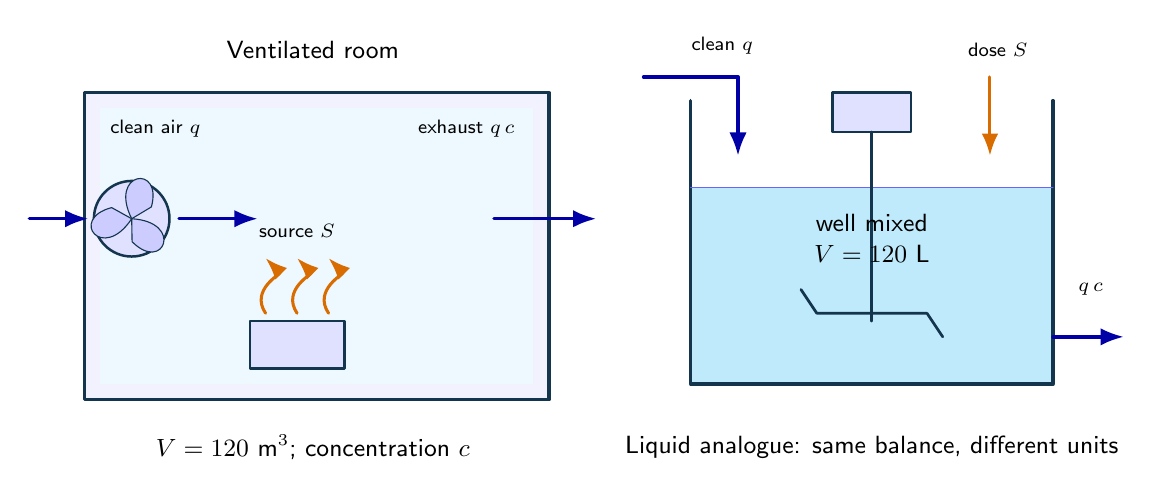
\begin{tikzpicture}[
font=\sffamily\small,>=Latex,line cap=round,line join=round,
wall/.style={draw=ink,line width=1.2pt,fill=blue!5},
water/.style={fill=cyan!25,draw=none},
metal/.style={draw=ink,fill=blue!12,line width=.9pt},
flow/.style={->,draw=blue!65!black,line width=1.2pt},
heat/.style={->,draw=orange!85!black,line width=1.1pt},
measure/.style={->,draw=teal!70!black,line width=.9pt},
dim/.style={<->,draw=ink!65,line width=.6pt},
spring/.style={draw=ink,decorate,decoration={coil,aspect=.5,segment length=4pt,amplitude=3pt}},
wire/.style={draw=ink,line width=1pt},
lab/.style={align=center,font=\sffamily\small},
smalllab/.style={align=center,font=\sffamily\scriptsize}]

\draw[wall](.3,.2)--(.3,4.1)--(6.2,4.1)--(6.2,.2)--cycle;
\fill[cyan!7](.5,.4)rectangle(6,3.9);
\draw[metal](.9,2.5)circle(.48);
\foreach \a in {0,120,240}{\draw[ink,fill=blue!20,rotate around={\a:(.9,2.5)}](.9,2.5)..controls(.6,3.1)and(1.3,3.2)..(1.15,2.65)--cycle;}
\draw[flow](-.4,2.5)--(.35,2.5);
\draw[flow](1.5,2.5)--(2.5,2.5);
\draw[flow](5.5,2.5)--(6.8,2.5);
\node[smalllab]at(1.2,3.65){clean air $q$};
\node[smalllab]at(5.15,3.65){exhaust $q\,c$};
\draw[metal](2.4,.6)rectangle(3.6,1.2);
\foreach \x in {2.6,3,3.4}{\draw[heat](\x,1.3)..controls(\x-.2,1.6)and(\x+.2,1.8)..(\x,2);}
\node[smalllab]at(3,2.35){source $S$};
\node[lab]at(3.2,4.65){Ventilated room};
\node[lab]at(3.2,-.4){$V=120$ m$^3$; concentration $c$};
\fill[water](8,.4)rectangle(12.6,2.9);
\draw[wall,fill=none](8,4)--(8,.4)--(12.6,.4)--(12.6,4);
\draw[blue!60](8,2.9)--(12.6,2.9);
\draw[flow](7.4,4.3)--(8.6,4.3)--(8.6,3.3);
\draw[flow](12.6,1)--(13.5,1);
\draw[metal](9.8,3.6)rectangle(10.8,4.1);
\draw[wire](10.3,3.6)--(10.3,1.2);
\draw[wire](9.6,1.3)--(11,1.3)(9.6,1.3)--(9.4,1.6)(11,1.3)--(11.2,1);
\draw[heat](11.8,4.3)--(11.8,3.3);
\node[smalllab]at(11.9,4.65){dose $S$};
\node[smalllab]at(8.4,4.7){clean $q$};
\node[smalllab,anchor=west]at(12.8,1.6){$q\,c$};
\node[lab]at(10.3,2.25){well mixed\\$V=120$ L};
\node[lab]at(10.3,-.4){Liquid analogue: same balance, different units};
\end{tikzpicture}
}\par{\small A ventilated room and a well-mixed liquid analogue share an inventory balance. The room uses m$^3$ and the liquid case uses L; do not mix their concentration or flow units. Equal inlet and outlet volume flows keep each inventory constant.}\end{center}
\begin{enumerate}
\item A well-mixed volume has $V=120$ m$^3$, source $S=360$ ppm m$^3$/min and ventilation $q$ in m$^3$/min. Derive the balance for excess concentration $c$ and the equilibrium and time constant at $q_0=3$.
\item Linearize $V\dot c=S-qc$ about $(S_0,q_0,c_0)=(360,3,120)$. Retain source and ventilation deviations as inputs. Give both transfer functions and the term neglected by linearization.
\item For nonzero $\delta c$, compare the discarded bilinear term with the retained term $q_0\delta c$. Give a useful local smallness condition and explain why it is not a complete error bound for a long transient.
\end{enumerate}
\vfill{\small\textbf{Submission.} Show the model, intermediate reasoning, units and a conclusion addressing the stated requirements.}

\newpage
\task{2}{Testing a linearization with progressively larger airflow steps}
Keep the source fixed and increase airflow from its nominal value. Compare exact equilibria, local predictions and the time needed to cross a concentration threshold.
\begin{enumerate}
\item Starting from 120 ppm, increase flow to 3.3 m$^3$/min while retaining the source. Derive the exact trajectory and the local-model prediction. Compare their equilibria and time constants.
\item Repeat the flow change with $q=6$. Find both equilibrium predictions and the exact time to reach 75 ppm. Explain whether the zero equilibrium predicted by the local model is physically attainable with a positive source.
\item Let $q=q_0(1+\varepsilon)$ with $\varepsilon>-1$. Derive exact and linearized equilibrium concentration, their absolute difference and their relative difference measured against the exact concentration. Evaluate the last quantity for $\varepsilon=0.1$ and 1.
\end{enumerate}
\vfill{\small\textbf{Submission.} Show the model, intermediate reasoning, units and a conclusion addressing the stated requirements.}

\newpage
\task{3}{A feedforward specification under source uncertainty}
The ventilation actuator has finite capacity. Design decisions must account both for the largest disturbance and for uncertainty in its magnitude.
\begin{center}\resizebox{\ifdim\width>.98\linewidth.98\linewidth\else\width\fi}{!}{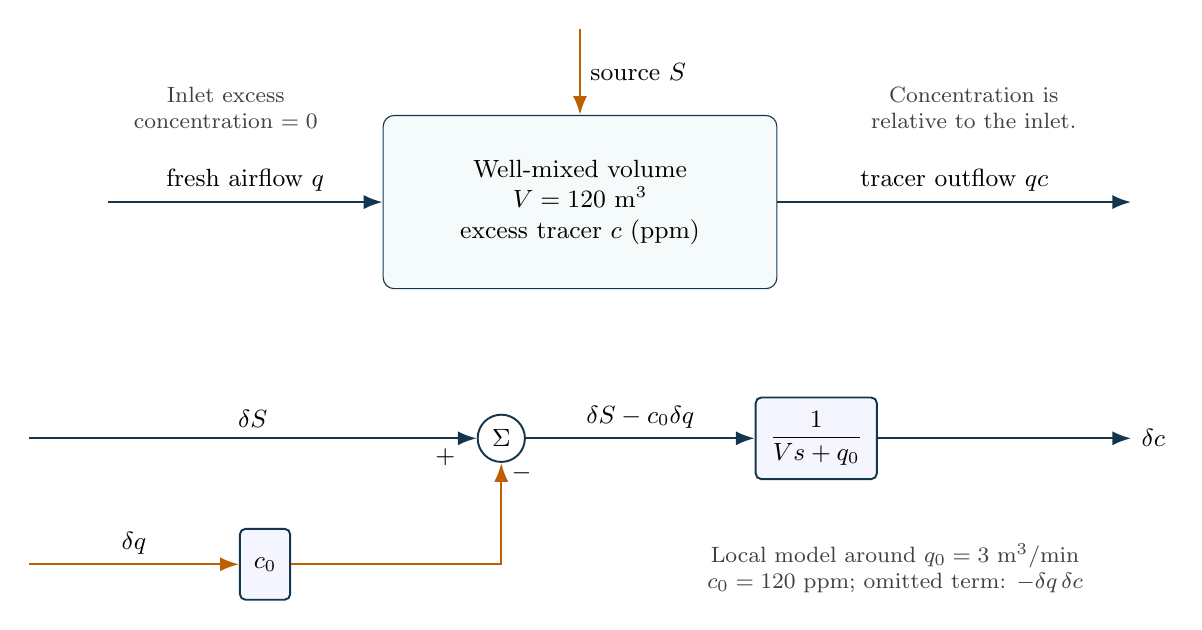
\begin{tikzpicture}[x=1cm,y=1cm,>=Latex,font=\small,
block/.style={draw=ink,fill=blue!4,rounded corners=2pt,minimum height=9mm,align=center,line width=.7pt,inner sep=5pt},
sum/.style={circle,draw=ink,fill=white,minimum size=6mm,inner sep=0pt,line width=.7pt},
sig/.style={->,draw=ink,line width=.85pt},
fb/.style={->,draw=teal!70!black,line width=.85pt},
dist/.style={->,draw=orange!75!black,line width=.85pt},
tap/.style={circle,fill=ink,inner sep=1.4pt},
note/.style={font=\footnotesize,align=center,text=black!75}]

\node[draw=ink,fill=teal!4,rounded corners,minimum width=50mm,minimum height=22mm,align=center](v)at(7,2.3){Well-mixed volume\\$V=120\ \mathrm{m^3}$\\excess tracer $c$ (ppm)};
\draw[sig](1,2.3)--node[above]{fresh airflow $q$}(v.west);
\draw[sig](v.east)--node[above]{tracer outflow $qc$}(14,2.3);
\draw[dist](7,4.5)--node[right]{source $S$}(v.north);
\node[note]at(2.5,3.5){Inlet excess\\concentration $=0$};
\node[note]at(12,3.5){Concentration is\\relative to the inlet.};
\node[sum](s)at(6,-.7){$\Sigma$};
\node[block](p)at(10,-.7){$\dfrac{1}{Vs+q_0}$};
\node[block](gain)at(3,-2.3){$c_0$};
\draw[sig](0,-.7)--node[above]{$\delta S$}node[pos=.93,below]{$+$}(s);
\draw[dist](0,-2.3)--node[above]{$\delta q$}(gain);
\draw[dist](gain)--(6,-2.3)--node[pos=.9,right]{$-$}(s);
\draw[sig](s)--node[above]{$\delta S-c_0\delta q$}(p);
\draw[sig](p)--(14,-.7)node[right]{$\delta c$};
\node[note]at(11,-2.35){Local model around $q_0=3\ \mathrm{m^3/min}$\\$c_0=120\ \mathrm{ppm}$; omitted term: $-\delta q\,\delta c$};

\end{tikzpicture}
}\par{\small The physical balance and its local two-input signal model. Airflow enters with a negative sign because increased ventilation removes excess tracer.}\end{center}
\begin{enumerate}
\item The target excess concentration is 100 ppm and the source rises from 360 to 480 ppm m$^3$/min. Find the required feedforward flows. If flow is limited to 4 m$^3$/min, find the final concentration after the source change.
\item At fixed flow $q=3.6$, the source is only known to lie in $[324,396]$. Find the equilibrium interval and the flow needed to guarantee an equilibrium no larger than 110 ppm under that source uncertainty.
\item Now use the uncertain source interval $[324,396]$ ppm m$^3$/min, require $c_\infty\le100$ ppm and retain maximum flow 4 m$^3$/min. Find the smallest constant flow that guarantees the requirement and the corresponding concentration interval.
\end{enumerate}
\vfill{\small\textbf{Submission.} Show the model, intermediate reasoning, units and a conclusion addressing the stated requirements.}

\newpage
\task{4}{Choosing the feedback sign and checking the resulting operating point}
The controller increases fresh airflow when excess concentration rises above its target. Use the nonlinear balance to check a controller designed from the local model.
\begin{enumerate}
\item Use $q=q_0+k(c-c_{ref})$ near $c_{ref}=c_0=120$. Derive the local closed-loop pole and choose $k$ for a 20 min time constant. Specify the units of $k$.
\item With the proportional law of Problem 4(a), a constant source increment of 60 ppm m$^3$/min occurs. Find the local steady concentration and flow deviations. Then find the exact positive equilibrium of the nonlinear balance and compare.
\item For the 60-unit source increment, calculate the exact equilibrium airflow with the specified proportional controller and check the limit $q\le4$. Explain why neither more proportional gain nor integral action can maintain 100 ppm when $S=480$ and this limit applies.
\end{enumerate}
\vfill{\small\textbf{Submission.} Show the model, intermediate reasoning, units and a conclusion addressing the stated requirements.}

\newpage
\task{5}{The same balance in a stirred dilution vessel}
Use the liquid analogue shown beside the room: an ideally mixed 120 L vessel receives clean water at $q$ L/min and a negligible-volume solute dose $S=360$ mg/min. Equal inlet and outlet flows maintain volume. Here $c_{ref}=120$ mg/L; the gains in part (a) use consistent L, mg and min units.
\begin{enumerate}
\item Let $e=c-c_{ref}$, $q=q_0+k_p e+z$, and $\dot z=k_i e$. Derive the linear characteristic polynomial. For $k_p=0.025$ and $k_i=0.0004$, calculate natural frequency and damping ratio.
\item Assume constant $S\ge0$, $q>0$ and $c(0)\ge0$. Prove that the exact concentration stays nonnegative and tends to $S/q$. Give two reasons a local model or this mixing model can be misleading in practice.
\item Map the room model to this vessel, state the new concentration units, and evaluate the feasibility of a 100 mg/L target when $S=480$ mg/min and $q\le4$ L/min. Explain the consequence for the proposed integral controller.
\end{enumerate}
\vfill{\small\textbf{Submission.} Show the model, intermediate reasoning, units and a conclusion addressing the stated requirements.}

\end{document}
